
%(BEGIN_QUESTION)
% Copyright 2006, Tony R. Kuphaldt, released under the Creative Commons Attribution License (v 1.0)
% This means you may do almost anything with this work of mine, so long as you give me proper credit

En \textit{strain gauge} er et mønster laget av tynn metallfilm som er konstruert for å øke motstanden når den strekkes og redusere motstanden når den komprimeres.  Strain gauges limes vanligvis på metallprøver under mekanisk testing, som en måte å registrere hvor mye tøyning som påføres metallprøven.  For å omsette motstanden i strain gaugen til et målbart spenningssignal, bygges strain gaugen vanligvis inn i én arm av en ``bro''-krets.

\vskip 10pt

Følgende brokrets bruker to strain gauges (én for å måle tøyning, den andre for temperaturkompensasjon), der tøyningen vises av voltmeteret i midten av broen.  Men kretsen har et problem.  I stedet for å vise en liten spenning som normalt, er voltmeteret ``pegged'' (drevet forbi normalt fullskalaområde) av en stor spenningsforskjell, med punkt {\bf B} positivt og punkt {\bf A} negativt som vist her:

$$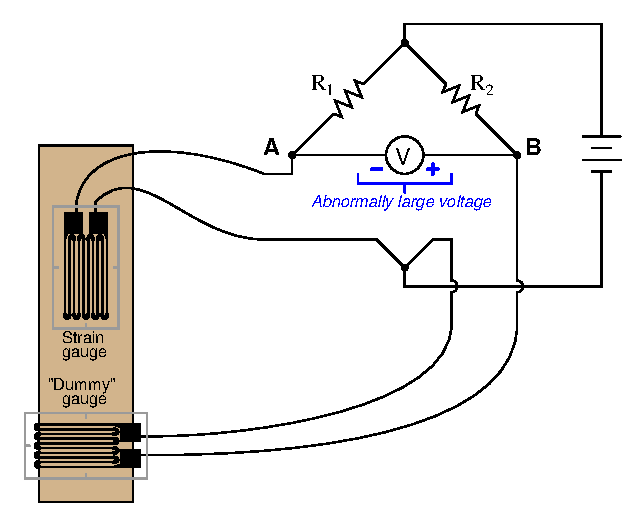
\includegraphics[width=15.5cm]{i00188x01.eps}$$

\goodbreak
Noe er galt i brokretsen, fordi denne spenningen er til stede selv uten fysisk belastning på prøven.  Identifiser hvilke av følgende feil som kan forårsake for høy spenning over voltmeteret, og hvilke som ikke kan det.  Vurder kun én feil om gangen (ingen flere samtidige feil):

% No blank lines allowed between lines of an \halign structure!
% I use comments (%) instead, so that TeX doesn't choke.

$$\vbox{\offinterlineskip
\halign{\strut
\vrule \quad\hfil # \ \hfil & 
\vrule \quad\hfil # \ \hfil & 
\vrule \quad\hfil # \ \hfil \vrule \cr
\noalign{\hrule}
%
% First row
{\bf Fault} & {\bf Possible} & {\bf Impossible} \cr
%
\noalign{\hrule}
%
% Another row
$R_1$ failed open &  &  \cr
%
\noalign{\hrule}
%
% Another row
$R_2$ failed open &  &  \cr
%
\noalign{\hrule}
%
% Another row
Strain gauge failed open &  &  \cr
%
\noalign{\hrule}
%
% Another row
Dummy gauge failed open &  &  \cr
%
\noalign{\hrule}
%
% Another row
$R_1$ failed shorted &  &  \cr
%
\noalign{\hrule}
%
% Another row
$R_2$ failed shorted &  &  \cr
%
\noalign{\hrule}
%
% Another row
Strain gauge failed shorted &  &  \cr
%
\noalign{\hrule}
%
% Another row
Dummy gauge failed shorted &  &  \cr
%
\noalign{\hrule}
%
% Another row
Voltage source dead &  &  \cr
%
\noalign{\hrule}
} % End of \halign 
}$$ % End of \vbox

\vskip 20pt \vbox{\hrule \hbox{\strut \vrule{} {\bf Suggestions for Socratic discussion} \vrule} \hrule}

\begin{itemize}
\item{} Identifiser hvilke grunnprinsipper i elektriske kretser som gjelder for hvert steg i analysen.  Vær forberedt på å forklare ``hvorfor'' for hvert steg, ikke bare beskrive stegene.
\item{} Forklar hvorfor de to strain gauge-elementene er limt ortogonalt (dvs. 90$^{o}$ i forhold til hverandre) på prøven.
\end{itemize}

\underbar{file i00188}
%(END_QUESTION)





%(BEGIN_ANSWER)

\noindent
{\bf Delvis svar:}

% No blank lines allowed between lines of an \halign structure!
% I use comments (%) instead, so that TeX doesn't choke.

$$\vbox{\offinterlineskip
\halign{\strut
\vrule \quad\hfil # \ \hfil & 
\vrule \quad\hfil # \ \hfil & 
\vrule \quad\hfil # \ \hfil \vrule \cr
\noalign{\hrule}
%
% First row
{\bf Fault} & {\bf Possible} & {\bf Impossible} \cr
%
\noalign{\hrule}
%
% Another row
$R_1$ failed open & $\surd$ &  \cr
%
\noalign{\hrule}
%
% Another row
$R_2$ failed open &  &  \cr
%
\noalign{\hrule}
%
% Another row
Strain gauge failed open &  & $\surd$ \cr
%
\noalign{\hrule}
%
% Another row
Dummy gauge failed open &  &  \cr
%
\noalign{\hrule}
%
% Another row
$R_1$ failed shorted &  &  \cr
%
\noalign{\hrule}
%
% Another row
$R_2$ failed shorted &  &  \cr
%
\noalign{\hrule}
%
% Another row
Strain gauge failed shorted &  &  \cr
%
\noalign{\hrule}
%
% Another row
Dummy gauge failed shorted &  &  \cr
%
\noalign{\hrule}
%
% Another row
Voltage source dead &  & $\surd$ \cr
%
\noalign{\hrule}
} % End of \halign 
}$$ % End of \vbox

%(END_ANSWER)





%(BEGIN_NOTES)

% No blank lines allowed between lines of an \halign structure!
% I use comments (%) instead, so that TeX doesn't choke.

$$\vbox{\offinterlineskip
\halign{\strut
\vrule \quad\hfil # \ \hfil & 
\vrule \quad\hfil # \ \hfil & 
\vrule \quad\hfil # \ \hfil \vrule \cr
\noalign{\hrule}
%
% First row
{\bf Fault} & {\bf Possible} & {\bf Impossible} \cr
%
\noalign{\hrule}
%
% Another row
$R_1$ failed open & $\surd$ &  \cr
%
\noalign{\hrule}
%
% Another row
$R_2$ failed open &  & $\surd$ \cr
%
\noalign{\hrule}
%
% Another row
Strain gauge failed open &  & $\surd$ \cr
%
\noalign{\hrule}
%
% Another row
Dummy gauge failed open & $\surd$ &  \cr
%
\noalign{\hrule}
%
% Another row
$R_1$ failed shorted &  & $\surd$ \cr
%
\noalign{\hrule}
%
% Another row
$R_2$ failed shorted & $\surd$ &  \cr
%
\noalign{\hrule}
%
% Another row
Strain gauge failed shorted & $\surd$ &  \cr
%
\noalign{\hrule}
%
% Another row
Dummy gauge failed shorted &  & $\surd$ \cr
%
\noalign{\hrule}
%
% Another row
Voltage source dead &  & $\surd$ \cr
%
\noalign{\hrule}
} % End of \halign 
}$$ % End of \vbox

Denne oppgaven hjelper studenter med å bygge ferdigheten i å eliminere usannsynlige feil, slik at de kan fokusere på det som er mest sannsynlig.  En viktig ferdighet i feilsøking er evnen til å vurdere sannsynligheten for ulike feilscenarioer.  Uten denne ferdigheten brukes ofte mye tid på lite sannsynlige feil.

For hvert feilscenario er det viktig å spørre studentene \textit{hvorfor} de mener feilen er mulig eller ikke.  Noen kan komme til riktig svar av feil grunn, så det er nyttig å utforske begrunnelsen bak hvert svar.

\filbreak

$$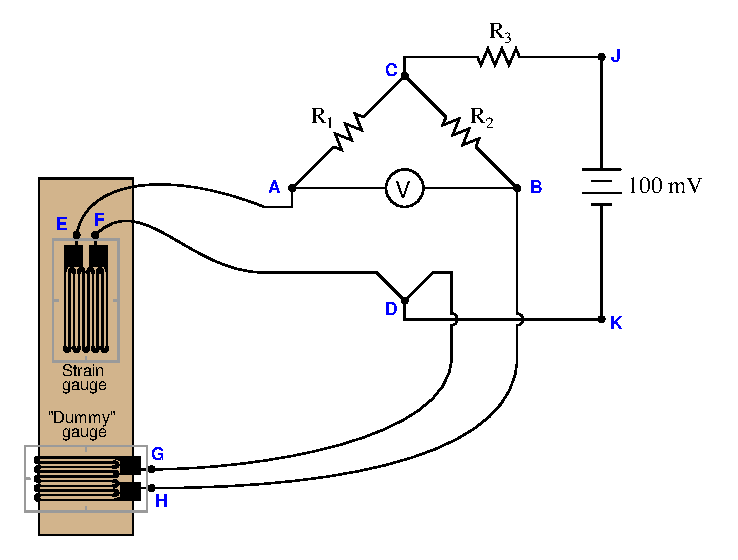
\includegraphics[width=15.5cm]{i00188x02.eps}$$

\vskip 20pt \vbox{\hrule \hbox{\strut \vrule{} {\bf Virtual Troubleshooting} \vrule} \hrule}

Denne oppgaven passer godt som ``Virtual Troubleshooting''-øvelse.  Presenter diagrammet for studentene, velg deretter en bestemt feil i tankene dine.  Presenter ett eller flere symptomer på denne feilen (noe en bruker eller operatør kan observere).  Studentene foreslår så diagnostiske tester for å identifisere type og plassering av feilen, som om de var teknikere i felt.  Din jobb er å oppgi hvilket resultat hver foreslåtte test ville gitt, og dokumentere resultatene synlig for alle.

Under og etter øvelsen er det nyttig å stille oppfølgingsspørsmål som:

\begin{itemize}
\item{} Hva forteller resultatet av siste test deg om feilen?
\item{} Hvis resultatet av siste test hadde vært annerledes, hva ville det da fortalt deg om feilen?
\item{} Er siste test den beste vi kunne gjort?
\item{} Hva ville vært optimal testrekkefølge for å finne feilen i færrest mulig steg?
\end{itemize}

%INDEX% Measurement, strain gauge

%(END_NOTES)

